\documentclass[12pt,aspectratio=169]{beamer}

\usetheme{metropolis}

\definecolor{mDarkBrown}{HTML}{FF5722}
\definecolor{mDarkTeal}{HTML}{263238}
\definecolor{mLightBrown}{HTML}{FF5722}

\usepackage{booktabs}
\usepackage{graphicx}
\usepackage{hyphenat}
\usepackage{multirow}
\usepackage{nicefrac}
\usepackage[normalem]{ulem}

\usepackage[weather]{ifsym}

\usepackage{pifont}
\newcommand{\cmark}{\ding{51}}
\newcommand{\xmark}{\ding{55}}

\usepackage{minted}
\usemintedstyle{tango}
\newminted[bash]{bash}{%
    autogobble,
    bgcolor=mDarkTeal!10,
    linenos
}
\newminted[py3]{python}{%
    python3,
    autogobble,
    bgcolor=mDarkTeal!10,
    linenos
}
\newminted[sql]{sql}{%
    autogobble,
    bgcolor=mDarkTeal!10,
    linenos
}

\usepackage{polyglossia}
\setdefaultlanguage[variant=british]{english}
\usepackage[english=british]{csquotes}

\defaultfontfeatures{Ligatures=TeX}
\setmainfont{Lucida Sans OT}
\setsansfont[Scale=MatchLowercase]{Lucida Sans OT}
\setmonofont[Scale=MatchLowercase]{Lucida Console DK}

\usepackage{mathspec}
\setmathsfont(Digits,Latin,Greek)[Numbers={Lining,Proportional}]{Lucida Bright Math OT}

\newcommand{\mat}[1]{\ensuremath{\mathbf{#1}}}

\newcommand{\R}{\ensuremath{\mathbb{R}}}

\newcommand{\E}[1]{\ensuremath{\mathbb{E}\!\left[ #1 \right]}}
\newcommand{\V}[1]{\ensuremath{\mathbb{V}\!\left[ #1 \right]}}
\newcommand{\Prob}[1]{\ensuremath{\Pr\!\left( #1 \right)}}
\newcommand{\Normal}[2]{\ensuremath{\mathcal{N}\!\left( #1, #2 \right)}}
\newcommand{\simiid}{\ensuremath{\overset{\text{\tiny i.i.d.}}{\sim}}}

\DeclareMathOperator{\logit}{logit}

\author{Gianluca Campanella}
\date{}



\title{Generalised linear models}

\begin{document}

\maketitle

\begin{frame}{Contents}
    \tableofcontents[hideallsubsections]
\end{frame}

\section{Regression models}

\begin{frame}{Regression models}
    Regression models explore associations between:
    \begin{itemize}
        \item A \alert{response} variable $\vec{y}$
        \item \alert{Explanatory} variables (or \alert{predictors})
              $\vec{x_{1}}, \ldots, \vec{x_{p}}$
    \end{itemize}
    \vfill\pause
    \begin{block}{Question}
        Do the $\vec{x_{1}}, \ldots, \vec{x_{p}}$ capture the
        \alert{variability} of $\vec{y}$?
    \end{block}
\end{frame}

\begin{frame}{Regression modelling steps}
    \begin{itemize}
        \item \alert{Formulation}
              \begin{enumerate}
                  \item Error distribution for the response $\vec{y}$
                  \item Combination of predictors
                  \item Link function \\[\bigskipamount]
              \end{enumerate}
        \item \alert{Estimation} of regression coefficients \\[\bigskipamount]
        \item \alert{Diagnostics} (does the model fit the data well?) \\[\bigskipamount]
        \item \alert{Selection} (can we improve the fit?)
    \end{itemize}
\end{frame}

\begin{frame}{Components of regression models}
    \begin{enumerate}[(1)]
        \item A model for the \alert{variability} of the response $\vec{y}$
              \begin{itemize}
                  \item $\vec{y}$ is continuous $\rightarrow$ normal distribution
                  \item $\vec{y}$ is dichotomous $\rightarrow$ binomial distribution \\[\bigskipamount]
              \end{itemize}
        \pause
        \item A \alert{combination of predictors} $\vec{x_{1}}, \ldots, \vec{x_{p}}$
              \begin{itemize}
                  \item Often linear, e.g.\ $2 \vec{x_{1}} + 3 \vec{x_{2}}$
                  \item $\beta_{1} = 2$ and $\beta_{2} = 3$ are
                        \alert{regression coefficients} \\[\bigskipamount]
              \end{itemize}
        \pause
        \item A \alert{link} between the two
              \begin{itemize}
                  \item Often depends on the model for the response
                  \item Linear regression:
                        $\E{\vec{y}} = 2 \vec{x_{1}} + 3 \vec{x_{2}}$
              \end{itemize}
    \end{enumerate}
\end{frame}

\begin{frame}{Predictors and response}
    \begin{block}{Predictors}
        \begin{itemize}
            \item Viewed as \alert{fixed} variables
            \item Assumed not to be affected by \alert{measurement error}
            \item[$\rightarrow$] `Independent' or `exogenous'
        \end{itemize}
    \end{block}
    \vfill
    \begin{block}{Response}
        \begin{itemize}
            \item \alert{Variability is modelled} \\
                  (but could also be attributed to other factors)
            \item[$\rightarrow$] `Dependent' or `endogenous'
        \end{itemize}
    \end{block}
\end{frame}

\section{Linear regression}

\begin{frame}{Simple linear regression}
    \begin{columns}[c]
        \begin{column}{0.5\textwidth}
            \centering
            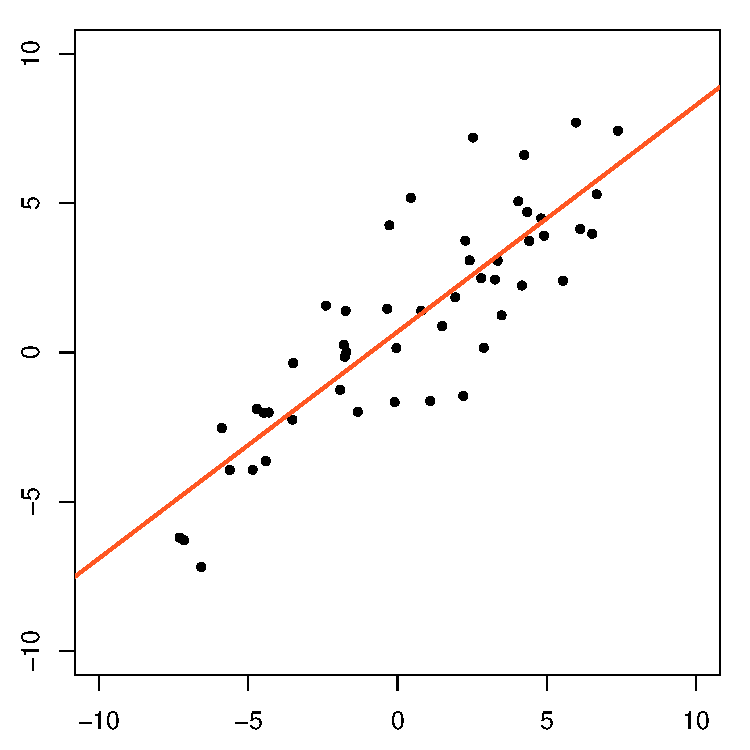
\includegraphics[width=\textwidth]{figures/lm}
        \end{column}
        \begin{column}{0.5\textwidth}
            {\small%
             For the $i^{\,\text{th}}$ observation:}
            \vspace{-1ex}
            \begin{center}
                $y_{i} = \beta_{0} + \beta_{1}\,x_{i} + \epsilon_{i}$ \\[\bigskipamount]
                \begin{tabular}{ll}
                    \toprule
                    $\beta_{0}$    & Intercept \\
                    $\beta_{1}$    & Slope \\
                    $\epsilon_{i}$ & Individual error term \\
                    \bottomrule
                \end{tabular}
            \end{center}
        \end{column}
    \end{columns}
\end{frame}

\begin{frame}[t]{Regression coefficients}
    \[
        y_{i} = \alert{\beta_{0}} + \alert{\beta_{1}}\,x_{i} + \epsilon_{i}
    \]
    \vfill
    \begin{description}
        \item[\textbf{Intercept}] Average $y$ when $x = 0$
        \item[\textbf{Slope}] Increase in $y$ for a one\hyp{}unit increase in $x$
    \end{description}
    \vfill
    The regression line passes through:\vspace{-1ex}
    \begin{itemize}
        \item The point $(0, \beta_{0})$
        \item The `centre' of the data $(\bar{\vec{x}}, \bar{\vec{y}})$
    \end{itemize}
\end{frame}

\begin{frame}[t]{Error term}
    \[
        y_{i} = \beta_{0} + \beta_{1}\,x_{i} + \alert{\epsilon_{i}}
    \]
    \vfill
    \begin{itemize}
        \item `Sucks up' unaccounted variation in $\vec{y}$
        \item Model assumptions are mostly on $\epsilon$
    \end{itemize}
\end{frame}

\begin{frame}[t]{Multiple linear regression}
    \only<1>{%
        {\small%
         For the $i^{\,\text{th}}$ observation:}
        \vspace{-1ex}
        \begin{center}
            $y_{i} = \beta_{0} + \sum_{j} \beta_{j}\,x_{ij} + \epsilon_{i}$ \\[\bigskipamount]
            \begin{tabular}{ll}
                \toprule
                $\beta_{0}$    & Intercept \\
                $\beta_{j}$    & Slopes \\
                $\epsilon_{i}$ & Individual error term \\
                \bottomrule
            \end{tabular}
        \end{center}
        \vfill
        \begin{description}
            \item[\textbf{Intercept}] Average $y$ when all $x_{\,\cdot\,j} = 0$
            \item[\textbf{Slopes}] Increase in $y$ for a one\hyp{}unit increase
                                   in $x_{\,\cdot\,j}$ \\
                                   \alert{all else being equal}
        \end{description}}
    \only<2>{%
        {\small
         In matrix form:}
        \vspace{-1ex}
        \begin{center}
            $\vec{y} = \mat{X} \vec{\beta} + \vec{\epsilon}$ \\[\bigskipamount]
            \begin{tabular}{ll}
                \toprule
                $\mat{X}$        & Design matrix\\
                $\vec{\beta}$    & Regression coefficients \\
                $\vec{\epsilon}$ & Error term \\
                \bottomrule
            \end{tabular}
        \end{center}}
\end{frame}

\begin{frame}{Gauss--Markov assumptions (plus one)}
    \begin{itemize}
        \item The relationship between $\vec{y}$ and $\mat{X}$ is linear
        \item The $\vec{x_{1}}, \ldots, \vec{x_{p}}$ are not collinear
        \item Exogeneity
              \begin{itemize}
                  \item Given $\mat{X}$, errors have mean 0
                  \item Since $\mat{X}_{i}$ is deterministic, it is uncorrelated
                        with $\epsilon_{i}$
              \end{itemize}
        \item Spherical errors
              \begin{itemize}
                  \item Errors have a fixed variance (homoscedasticity)
                  \item Errors are uncorrelated between observations
                        (no autocorrelation)
              \end{itemize}
        \item (Given $\mat{X}$, errors are normally distributed)
    \end{itemize}
\end{frame}

\begin{frame}[t]{Model fitting by maximum likelihood}
    \begin{center}
        $Y_{i} \sim \Normal{\mu_{i}}{\sigma^{2}}$
        \quad
        where
        \quad
        $\mu_{i} = \beta_{0} + \sum_{j} \beta_{j}\,x_{ij}$
    \end{center}
    \vfill
    \only<1>{%
        \begin{description}
            \item[$\beta_{j}$] `True' values (\alert{fixed but unknown})
            \item[$\hat{\beta}_{j}$] Our estimates for the $\beta_{j}$
                                     (\alert{computed from the data})
        \end{description}
        \vfill
        Given some values for the $\hat{\beta}_{j}$\ldots\vspace{-1ex}
        \begin{itemize}
            \item We can write down the probability of observing each $Y_{i}$
                  alone
            \item Since the $Y_{i}$ are independent by assumption, we can write
                  down the \alert{joint} probability of observing the $Y_{i}$
                  together
            \item[$\rightarrow$] $f\,( \vec{y}\,|\,\hat{\beta}_{j} )$ is the
                                 probability of the data
                                 \alert{given the parameters}
        \end{itemize}}
    \only<2>{%
        \begin{block}{Maximum likelihood principle}
            \begin{itemize}
                \item Consider instead the \alert{likelihood function}
                      $f\,( \hat{\beta}_{j}\,|\,\vec{y} )$
                \item Same as $f\,( \vec{y}\,|\,\hat{\beta}_{j} )$, but
                      interpreted as the probability of certain parameter values
                      \alert{given the data}
                \item[$\rightarrow$] Can optimise to estimate the $\hat{\beta}_{j}$
            \end{itemize}
        \end{block}}
\end{frame}

\begin{frame}{Hypothesis testing for parameters}
    How do we know the \alert{estimates} $\hat{\beta}_{j}$ are not just random
    fluctuations?
    \vfill\pause
    \begin{center}
        Additional assumption: $\epsilon_{i} \simiid \Normal{0}{\sigma^{2}}$ \\[\bigskipamount]
        $\downarrow$ \\[\bigskipamount]
    \end{center}
    \begin{itemize}
        \item Define confidence intervals for $\hat{\beta}_{j}$
        \item Test $H_{0}$ that $\hat{\beta}_{j} = 0$ (no effect)
    \end{itemize}
\end{frame}

\begin{frame}{Diagnostics for linear regression}
    \begin{center}
        \begin{tabular}{llp{0.5\textwidth}}
            \toprule
            \textbf{Assumption violated} & \textbf{Severity} & \textbf{Causes} \\
            \midrule
            Linearity or additivity & ++++ & Model misspecification \\[\medskipamount]
            Independence            & +++  & Autocorrelation \newline (typical of time series) \\[\medskipamount]
            Homoscedasticity        & ++   & $\sigma^{2}$ changes over the range of $\vec{y}$ \\[\medskipamount]
            Normality               & +    & Outliers \\
            \bottomrule
        \end{tabular}
    \end{center}
\end{frame}

\begin{frame}{Many datasets, one regression line}
    \begin{center}
        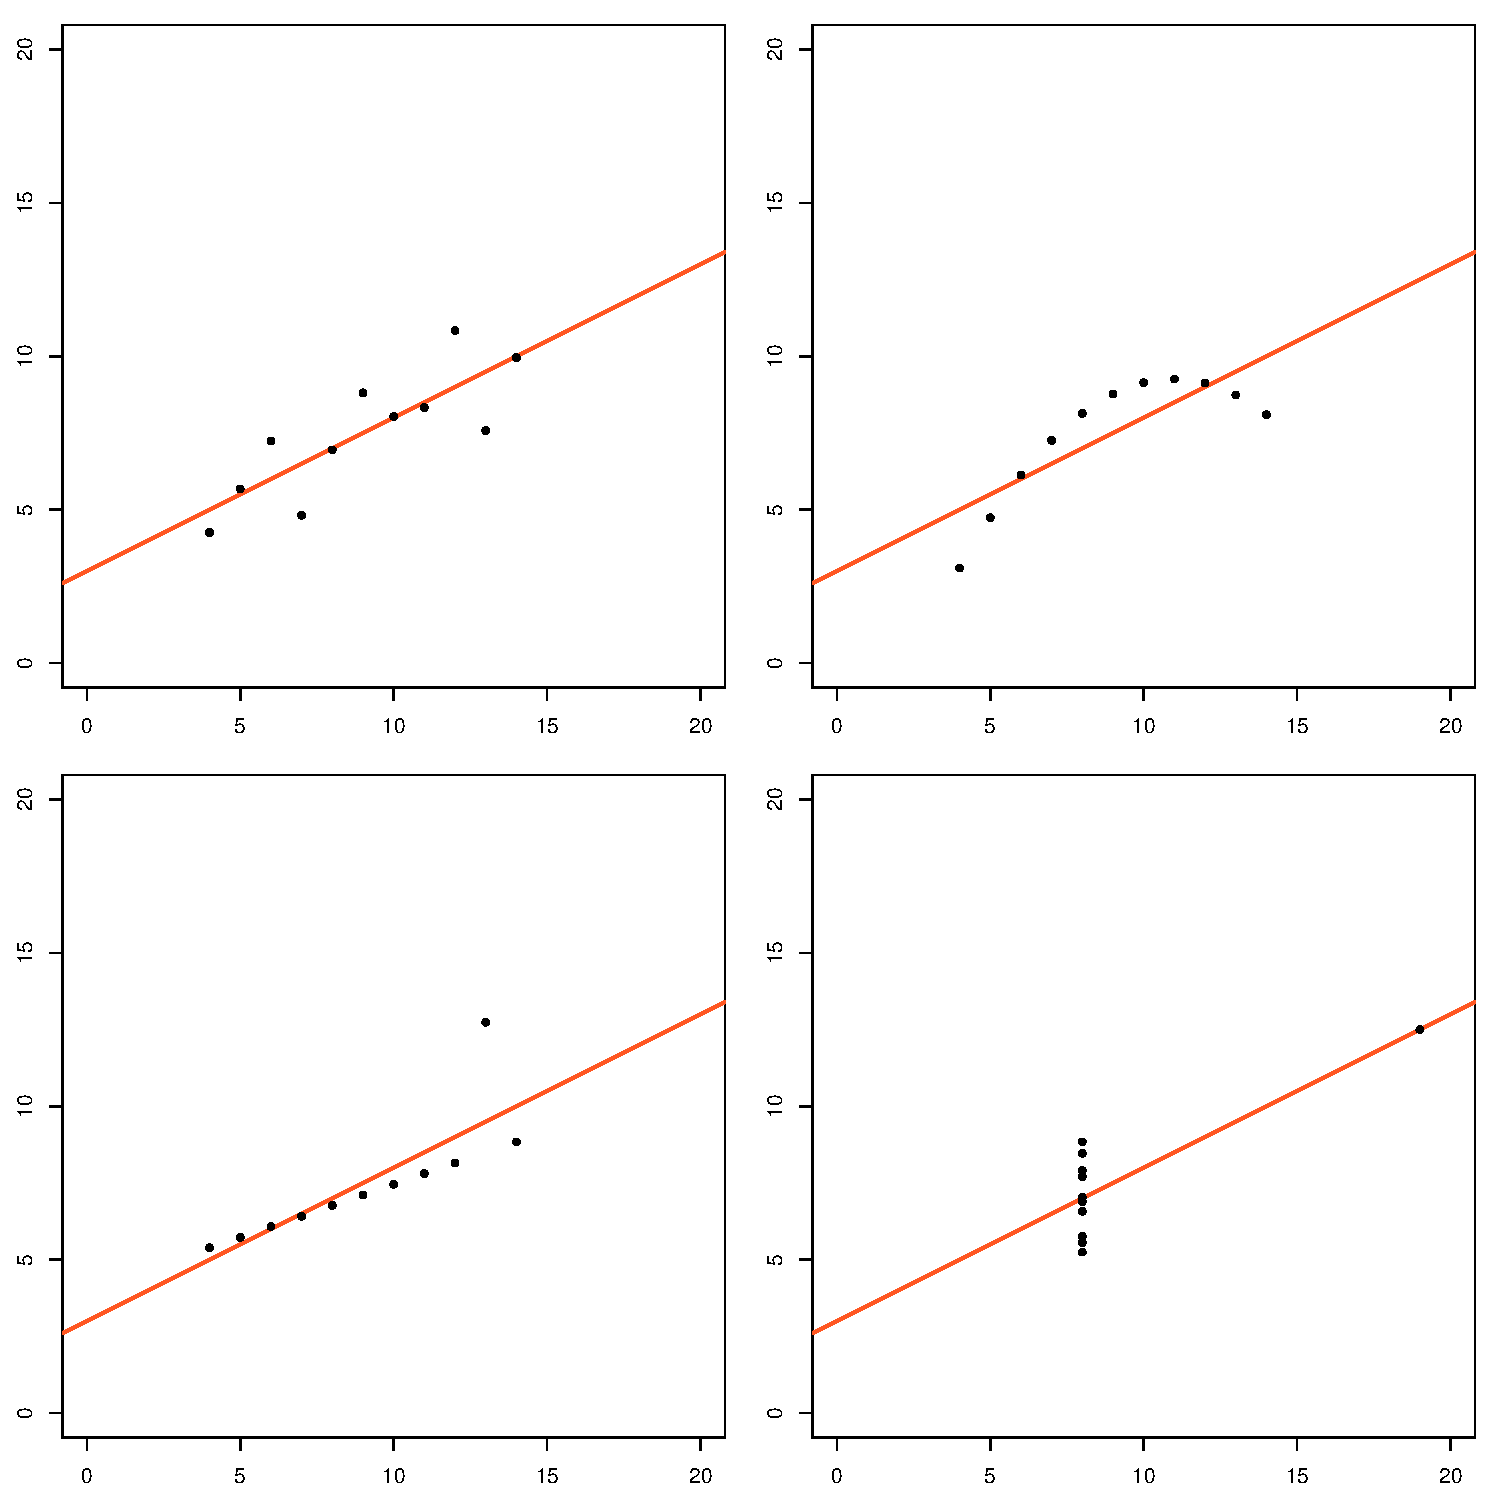
\includegraphics[height=0.8\textheight]{figures/anscombe}
    \end{center}
\end{frame}

\section{Logistic regression}

\begin{frame}{Classification problems}
    \begin{center}
        What happens if the outcome $\vec{y}$ is dichotomous?
    \end{center}
    \vfill\pause
    We can model the \alert{probability}
    \[
        \Prob{y_{i} = 1 \,\left|\,\vec{x}_{i} \right.\!} = p_{i}\text{,}
    \]
    i.e.\ the probability of belonging to some non\hyp{reference} category, as a
    function of the predictors $\vec{x_{1}}, \ldots, \vec{x_{p}}$
    \vfill
    \begin{flushright}
        \ldots but how?
    \end{flushright}
\end{frame}

\begin{frame}{Logistic regression}
    \begin{block}{Idea}
        Transform the linear predictor to lie on the unit interval \\[\bigskipamount]
        {\small%
         For the $i^{\,\text{th}}$ observation:}
        \[
            \logit\!\left( p_{i} \right)
            = \log\!\left( \frac{p_{i}}{1 - p_{i}} \right)
            = \beta_{0} + \sum_{j} \beta_{j} x_{ij} + \epsilon
        \]
        $\beta_{0}, \ldots, \beta_{p}$ represent the
        \alert{log odds ratios} between classes
    \end{block}
\end{frame}

\begin{frame}{Probability and odds}
    \begin{columns}[c]
        \begin{column}{0.5\textwidth}
            \centering
            \[
                \logit\!\left( p \right) = \log\!\left( \frac{p}{1 - p} \right)
            \]
            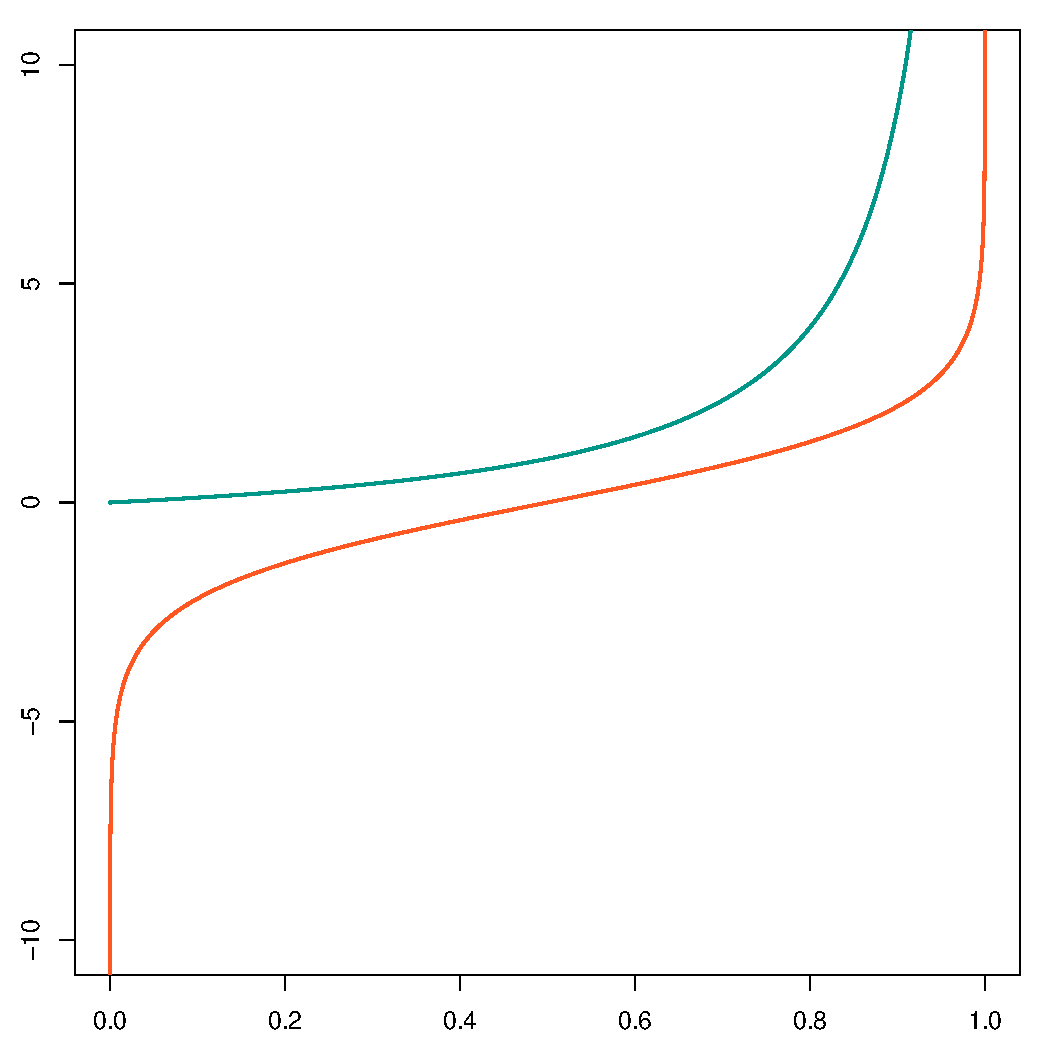
\includegraphics[width=0.8\textwidth]{figures/logit}
        \end{column}
        \begin{column}{0.5\textwidth}
            Throw a fair die. \\
            How often will you get a $1$?
            \begin{block}{Probability}
                \[
                    p = \frac{1}{6} \approx 16.67\% \text{ of the time}
                \]
            \end{block}
            \vspace{-0.5em}
            \begin{block}{Odds}
                \[
                    \frac{p}{1 - p} = \frac{1/6}{5/6} = \frac{1}{5} = 0.2
                \]
                {\footnotesize%
                 (once for every $5$ times you don't)}
            \end{block}
        \end{column}
    \end{columns}
\end{frame}

\begin{frame}[t]{Odds ratio}
    \only<1>{%
        \[
            \text{OR} = \frac{\text{odds in some group ($y = 1$)}}
                             {\text{odds in a reference group ($y = 0$)}}
        \]}
    \only<2>{%
        \begin{block}{Example}
            \[
                \text{OR} = \frac{\text{odds of smoking in lung cancer patients}}
                                 {\text{odds of smoking in cancer\hyp{}free individuals}}
            \]
        \end{block}
        \vfill
        \begin{block}{Interpretation}
            \[
                \text{OR}
                \begin{cases}
                    < 1 & \text{smoking is \alert{less likely}} \\
                    = 1 & \text{smoking is \alert{no more likely} in lung cancer patients} \\
                    > 1 & \text{smoking is \alert{more likely}}
                \end{cases}
            \]
        \end{block}}
\end{frame}

\begin{frame}{Logistic regression recap}
    \begin{block}{Model}
        \begin{itemize}
            \item Outcome is the \alert{probability} of being in some
                  non\hyp{}reference class
            \item Regression coefficients represent \alert{log odds ratios}
        \end{itemize}
    \end{block}
    \vfill
    \begin{block}{Interpretation of coefficients}
        \begin{itemize}
            \item $\exp\!\left( \beta \right)$ is the \alert{odds ratio} between
                  $y = 0$ and $y = 1$
            \item $\text{OR} = 1$ is the threshold corresponding to no effect
        \end{itemize}
    \end{block}
\end{frame}

\end{document}

